% $Author: oscar $
% $Date: 2009-09-15 16:53:48 +0200 (Tue, 15 Sep 2009) $
% $Revision: 29111 $
%=================================================================
\ifx\wholebook\relax\else
% --------------------------------------------
% Lulu:
	\documentclass[a4paper,10pt,twoside]{book}
	\usepackage[
		papersize={6.13in,9.21in},
		hmargin={.815in,.815in},
		vmargin={.98in,.98in},
		ignoreheadfoot
	]{geometry}
	\usepackage[hangul]{kotex}
	% $Author: oscar $
% $Date: 2009-09-13 20:58:29 +0200 (Sun, 13 Sep 2009) $
% $Revision: 29070 $
%=============================================================
% NB: documentclass must be set in main document.
% Allows book to be generated in multiple formats.
%=============================================================
%:Packages
\usepackage[T1]{fontenc}  %%%%%really important to get the code directly in the text!
\usepackage{palatino}
\usepackage{ifthen}
\usepackage{graphicx}
\graphicspath{{figures/}}
\usepackage{xspace}
\usepackage{makeidx}
\usepackage{isodateo} % enable \isodate
\usepackage{amssymb,textcomp}
%=============================================================
%:More packages
%\usepackage[english]{babel}
%\usepackage{lmodern}
%\usepackage[scaled=0.85]{helvet}
%\usepackage{microtype}
%\usepackage{theorem}
%\usepackage{float}
%\usepackage{longtable}
%\usepackage[nottoc]{tocbibind}
%\usepackage{multicol}
%\usepackage{booktabs}	% book-style tables
%\usepackage{topcapt}	% enables \topcaption
%\usepackage{multirow}
%\usepackage{tabularx}
%\usepackage{alltt}
\usepackage[usenames,dvipsnames]{color}
%\usepackage[hang]{subfigure}\makeatletter\def\p@subfigure{\thefigure\,}\makeatother
%\usepackage{rotating}
%\usepackage{enumitem}	% apb: allows more control over tags in enumerations
%\usepackage{verbatim}     % for comment environment
%\usepackage{varioref}	% for page references that work
%\usepackage{needspace}
%\usepackage[newparttoc]{titlesec}
%\usepackage{titletoc}
%\usepackage{wrapfig}
\usepackage[
	colorlinks=true,
	linkcolor=black,
	urlcolor=black,
	citecolor=black
]{hyperref}   % should come last
%=============================================================
%:URL style
\makeatletter
\def\url@leostyle{%
  \@ifundefined{selectfont}{\def\UrlFont{\sf}}{\def\UrlFont{\sffamily}}}
\makeatother
\urlstyle{leo}
%=============================================================
%:Booleans
\newboolean{lulu}
\setboolean{lulu}{false}
\newcommand{\ifluluelse}[2]{\ifthenelse{\boolean{lulu}}{#1}{#2}}
%=============================================================
%:Editorial comment macros
\newcommand{\nnbb}[2]{
  \fbox{\bfseries\sffamily\scriptsize#1}
  {\sf\small$\blacktriangleright$\textit{#2}$\blacktriangleleft$}
}
\newcommand{\on}[1]{\nnbb{Oscar}{#1}}
\newcommand{\here}{\nnbb{CONTINUE}{HERE}}
%=============================================================
%:Abbreviation macros
\newcommand{\ie}{\emph{i.e.},\xspace}
\newcommand{\eg}{\emph{e.g.},\xspace}
\newcommand{\etc}{\emph{etc.}\xspace}
\newcommand{\etal}{\emph{et al.}\xspace}
\newcommand{\straightquote}{"}
\newcommand{\sba}{\url{SquareBracketAssociates.org}\xspace}
%=============================================================
%:Patterns
% \newcommand{\pattern}[2]{\newpage\section{{\sf #1}}\label{pat:#2}}
% \newcommand{\pattern}[2]{\newpage\index{#1 (Pattern)}\section{#1}\label{pat:#2}}
\newcommand{\pattern}[2]{\cleardoublepage\index{#1 (패턴)}\section{#1}\label{pat:#2}}
\newcommand{\thumbnail}[2]{\index{#1 (패턴)}\subsection{#1}\label{pat:#2}}
\newcommand{\thumblang}[2]{\index{#1 (패턴 랭귀지)}\subsection{#1}\label{pat:#2}}
\newcommand{\variant}[1]{{\emph{#1}}\xspace}
% \newcommand{\problem}[1]{\subsection*{Problem}\emph{#1}}
\newcommand{\intent}[1]{\paragraph{의도}\emph{#1}}
\newcommand{\problem}[1]{\paragraph{문제}\emph{#1}}
\newcommand{\solution}[1]{\paragraph{해결}\emph{#1}}
\newcommand{\discussion}[0]{\paragraph{토론}}
\newcommand{\cmd}[1]{{\tt #1}\xspace}
%=============================================================
%:Environments
\newenvironment{bulletlist}{\begin{itemize}\setlength{\itemsep}{0ex}}
{\end{itemize}}
%=============================================================
%:Cross reference macros
\newcommand{\chalabel}[1]{\label{cha:#1}}
\newcommand{\seclabel}[1]{\label{sec:#1}}
\newcommand{\figlabel}[1]{\label{fig:#1}}
\newcommand{\tablabel}[1]{\label{tab:#1}}
\newcommand{\rulelabel}[1]{\label{rule:#1}}
\newcommand{\eglabel}[1]{\label{eg:#1}}
\newcommand{\scrlabel}[1]{\label{scr:#1}}
\newcommand{\mthlabel}[1]{\label{mth:#1}}
\newcommand{\clslabel}[1]{\label{cls:#1}}
\newcommand{\faqlabel}[1]{\label{faq:#1}}
%\newcommand{\charef}[1]{Chapter~\ref{cha:#1}\xspace}
%\newcommand{\secref}[1]{Section~\ref{sec:#1}\xspace}
\newcommand{\figref}[1]{Figure~\ref{fig:#1}\xspace}
% \newcommand{\patpgref}[2]{\hyperref[pat:#2]{\sf #1} [p.~\pageref{pat:#2}]\xspace}
\newcommand{\patpgref}[2]{\index{#1 (Pattern)}\hyperref[pat:#2]{#1} [p.~\pageref{pat:#2}]\xspace}
\newcommand{\patlangpgref}[2]{\index{#1 (Pattern language)}\hyperref[pat:#2]{#1} [p.~\pageref{pat:#2}]\xspace}
% \newcommand{\patref}[2]{\hyperref[pat:#2]{\sf #1}\xspace}
\newcommand{\patref}[2]{\index{#1 (Pattern)}\hyperref[pat:#2]{#1}\xspace}
\newcommand{\patlangref}[2]{\index{#1 (Pattern language)}\hyperref[pat:#2]{#1}\xspace}
% \newcommand{\charef}[2]{\hyperref[cha:#2]{\underline{\sf #1}}\xspace}
% \newcommand{\charef}[2]{\hyperref[cha:#2]{\sf #1}\xspace}
\newcommand{\charef}[2]{\index{#1 (Pattern cluster)}\hyperref[cha:#2]{#1}\xspace}
% \newcommand{\chapgref}[2]{\hyperref[cha:#2]{\sf #1} [p.~\pageref{cha:#2}]\xspace}
\newcommand{\chapgref}[2]{\index{#1 (Pattern cluster)}\hyperref[cha:#2]{#1} [p.~\pageref{cha:#2}]\xspace}
%\newcommand{\Figref}[1]{Figure~\ref{fig:#1}\xspace}
%\newcommand{\appref}[1]{Appendix~\ref{app:#1}\xspace}
%\newcommand{\tabref}[1]{Table~\ref{tab:#1}\xspace}
%\newcommand{\ruleref}[1]{\ref{rule:#1}\xspace}
%\newcommand{\egref}[1]{example~\ref{eg:#1}\xspace}
%\newcommand{\Egref}[1]{Example~\ref{eg:#1}\xspace}
%\newcommand{\scrref}[1]{script~\ref{scr:#1}\xspace}
%\newcommand{\Scrref}[1]{Script~\ref{scr:#1}\xspace}
%\newcommand{\tscrref}[1]{the script~\ref{scr:#1}\xspace}
%\newcommand{\Tscrref}[1]{The script~\ref{scr:#1}\xspace}
%\newcommand{\mthref}[1]{method~\ref{mth:#1}\xspace}
%\newcommand{\mthsref}[1]{methods~\ref{mth:#1}\xspace}
%\newcommand{\Mthref}[1]{Method~\ref{mth:#1}\xspace}
%\newcommand{\tmthref}[1]{the method~\ref{mth:#1}\xspace}
%\newcommand{\Tmthref}[1]{The method~\ref{mth:#1}\xspace}
%\newcommand{\clsref}[1]{class~\ref{cls:#1}\xspace}
%\newcommand{\tclsref}[1]{the class~\ref{cls:#1}\xspace}
%\newcommand{\Tclsref}[1]{The class~\ref{cls:#1}\xspace}
%=============================================================
%:Page Layout
\setlength{\headsep}{1cm}
%=============================================================
%:Menu item macro
%\definecolor{lightgray}{gray}{0.89}
%\newcommand{\menu}[1]{{%
%	\setlength{\fboxsep}{0pt}%
%	\colorbox{lightgray}{{{\upshape\sffamily\strut \,#1\,}}}}}
%\newcommand{\go}{\,$\triangleright$\,}
%\newcommand{\short}[1]{\mbox{{\sc cmd}\hspace{0.08em}--\hspace{0.09em}#1}\xspace}
%\newcommand{\button}[1]{{%
%	\setlength{\fboxsep}{0pt}%
%	\fbox{{\upshape\sffamily\strut \,#1\,}}}}
%\newcommand{\toolsflap}{\textit{Tools} flap\xspace}
%=============================================================
%:Section depth
%\setcounter{secnumdepth}{2}
%
%\DeclareGraphicsExtensions{.pdf, .jpg, .png}
%=============================================================
%:PDF setup
\hypersetup{
   pdftitle={Object-Oriented Reengineering Patterns},
   pdfauthor={Serge Demeyer, St\'ephane Ducasse, Oscar Nierstrasz},
   pdfkeywords={Reengineering, Object-Oriented Programming, Patterns},
   pdfsubject={Computer Science}
}
%=============================================================
%:Page layout and appearance
%\renewcommand{\chaptermark}[1]{\markboth{#1}{}}
%\renewcommand{\sectionmark}[1]{\markright{\thesection\ #1}}
%\renewpagestyle{plain}[\small\itshape]{%
%	\setheadrule{0pt}%
%	\sethead[][][]{}{}{}%
%	\setfoot[][][]{}{}{}}
%\renewpagestyle{headings}[\small\itshape]{%
%	\setheadrule{0pt}%
%	\setmarks{chapter}{section}%
%	\sethead[\thepage][][\chaptertitle]{\sectiontitle}{}{\thepage}%
%	\setfoot[][][]{}{}{}}
%=============================================================
%:Title section setup and TOC numbering depth
%\setcounter{secnumdepth}{1}
%\setcounter{tocdepth}{1}
%\titleformat{\part}[display]{\centering}{\huge\partname\ \thepart}{1em}{\Huge\textbf}[]
%\titleformat{\chapter}[display]{}{\huge\chaptertitlename\ \thechapter}{1em}{\Huge\raggedright\textbf}[]
%\titlecontents{part}[3pc]{%
%		\pagebreak[2]\addvspace{1em plus.4em minus.2em}%
%		\leavevmode\large\bfseries}
%	{\contentslabel{3pc}}{\hspace*{-3pc}}
%	{}[\nopagebreak]
%\titlecontents{chapter}[3pc]{%
%		\pagebreak[0]\addvspace{1em plus.2em minus.2em}%
%		\leavevmode\bfseries}
%	{\contentslabel{3pc}}{}
%	{\hfill\contentspage}[\nopagebreak]
%\dottedcontents{section}[3pc]{}{3pc}{1pc}
%\dottedcontents{subsection}[3pc]{}{0pc}{1pc}
%\let\origdoublepage\cleardoublepage
%\newcommand{\clearemptydoublepage}{%
%  \clearpage
%  {\pagestyle{empty}\origdoublepage}}
%\let\cleardoublepage\clearemptydoublepage % see http://www.tex.ac.uk/cgi-bin/texfaq2html?label=patch
%=============================================================
%:Listings package configuration
\newcommand{\caret}{\makebox{\raisebox{0.4ex}{\footnotesize{$\wedge$}}}}
% \newcommand{\escape}{{\sf \textbackslash}}
\definecolor{source}{gray}{0.95}
\usepackage{listings}
\lstdefinelanguage{Smalltalk}{
  morestring=[d]',
% Adapt this to other languages!
%  morecomment=[s]{"}{"},
  alsoletter={\#:},
  %escapechar={!},
  literate=
    {BANG}{!}1
%    {UNDERSCORE}{\_}1
    {\\st}{Smalltalk}9 % convenience -- in case \st occurs in code
    % {'}{{\textquotesingle}}1 % replaced by upquote=true in \lstset
%    {_}{{$\leftarrow$}}1
    {>>>}{{\sep}}1
    {^}{{$\uparrow$}}1
    {~}{{$\sim$}}1
    {-}{{\sf -\hspace{-0.13em}-}}1  % the goal is to make - the same width as +
    {+}{\raisebox{0.08ex}{+}}1		% and to raise + off the baseline to match -
    {-->}{{\quad$\longrightarrow$\quad}}3
	, % Don't forget the comma at the end!
  tabsize=4
}[keywords,comments,strings]

\lstset{language=Smalltalk,
	basicstyle=\sffamily,
	keywordstyle=\color{black}\bfseries,
	% stringstyle=\ttfamily, % Ugly! do we really want this? -- on
	mathescape=true,
	showstringspaces=false,
	keepspaces=true,
	breaklines=true,
	breakautoindent=true,
	backgroundcolor=\color{source},
	lineskip={-1pt}, % Ugly hack
	upquote=true, % straight quote; requires textcomp package
	columns=fullflexible} % no fixed width fonts
% \newcommand{\ct}{\lstinline[mathescape=false,basicstyle={\sffamily\upshape}]}
\newcommand{\ct}{\lstinline[mathescape=false,backgroundcolor=\color{white},basicstyle={\sffamily\upshape}]}
\newcommand{\lct}[1]{{\textsf{\textup{#1}}}}
%\newcommand{\scat}[1]{\emph{\textsf{#1}}\xspace}
%\newcommand{\prot}[1]{\emph{\textsf{#1}}\xspace}
% NB: No argument!
\lstnewenvironment{code}[0]{%
	\lstset{%
		% frame=lines,
		frame=single,
		framerule=0pt,
		mathescape=false
	}
}{}
%\def\ignoredollar#1{}
%=============================================================
%:Reserving space
%\newcommand{\needlines}[1]{\Needspace{#1\baselineskip}}
%=============================================================
%:Indexing macros
% Macros ending with "ind" generate text as well as an index entry
% Macros ending with "index" *only* generate an index entry
\newcommand{\ind}[1]{\index{#1}#1\xspace} % plain text
\newcommand{\subind}[2]{\index{#1!#2}#2\xspace} % show #2, subindex under #1
\newcommand{\emphind}[1]{\index{#1}\emph{#1}\xspace} % emph #1
\newcommand{\emphsubind}[2]{\index{#1!#2}\emph{#2}\xspace} % show emph #2, subindex under #1
\newcommand{\patind}[1]{\index{#1@#1 (pattern)}\ct{#1}\xspace} % pattern
\newcommand{\seeindex}[2]{\index{#1|see{#2}}} % #1, see #2
%\newcommand{\boldidx}[1]{{\bf #1}} % breaks hyperlink
%\newcommand{\indmain}[1]{\index{#1}#1\xspace} 
%\newcommand{\emphsubindmain}[2]{\index{#1!#2}\emph{#2}\xspace} % subindex, main entry
%\newcommand{\subindmain}[2]{\index{#1!#2}#2\xspace} % subindex, main entry
%\newcommand{\clsindmain}[1]{\index{#1!\#@(class)}\ct{#1}\xspace} % class main
%\newcommand{\indexmain}[1]{\index{#1}} 
%=============================================================
\parskip 1ex
%=============================================================

	\pagestyle{headings}
	\setboolean{lulu}{true}
% --------------------------------------------
% A4:
%	\documentclass[a4paper,11pt,twoside]{book}
%	% $Author: oscar $
% $Date: 2009-09-13 20:58:29 +0200 (Sun, 13 Sep 2009) $
% $Revision: 29070 $
%=============================================================
% NB: documentclass must be set in main document.
% Allows book to be generated in multiple formats.
%=============================================================
%:Packages
\usepackage[T1]{fontenc}  %%%%%really important to get the code directly in the text!
\usepackage{palatino}
\usepackage{ifthen}
\usepackage{graphicx}
\graphicspath{{figures/}}
\usepackage{xspace}
\usepackage{makeidx}
\usepackage{isodateo} % enable \isodate
\usepackage{amssymb,textcomp}
%=============================================================
%:More packages
%\usepackage[english]{babel}
%\usepackage{lmodern}
%\usepackage[scaled=0.85]{helvet}
%\usepackage{microtype}
%\usepackage{theorem}
%\usepackage{float}
%\usepackage{longtable}
%\usepackage[nottoc]{tocbibind}
%\usepackage{multicol}
%\usepackage{booktabs}	% book-style tables
%\usepackage{topcapt}	% enables \topcaption
%\usepackage{multirow}
%\usepackage{tabularx}
%\usepackage{alltt}
\usepackage[usenames,dvipsnames]{color}
%\usepackage[hang]{subfigure}\makeatletter\def\p@subfigure{\thefigure\,}\makeatother
%\usepackage{rotating}
%\usepackage{enumitem}	% apb: allows more control over tags in enumerations
%\usepackage{verbatim}     % for comment environment
%\usepackage{varioref}	% for page references that work
%\usepackage{needspace}
%\usepackage[newparttoc]{titlesec}
%\usepackage{titletoc}
%\usepackage{wrapfig}
\usepackage[
	colorlinks=true,
	linkcolor=black,
	urlcolor=black,
	citecolor=black
]{hyperref}   % should come last
%=============================================================
%:URL style
\makeatletter
\def\url@leostyle{%
  \@ifundefined{selectfont}{\def\UrlFont{\sf}}{\def\UrlFont{\sffamily}}}
\makeatother
\urlstyle{leo}
%=============================================================
%:Booleans
\newboolean{lulu}
\setboolean{lulu}{false}
\newcommand{\ifluluelse}[2]{\ifthenelse{\boolean{lulu}}{#1}{#2}}
%=============================================================
%:Editorial comment macros
\newcommand{\nnbb}[2]{
  \fbox{\bfseries\sffamily\scriptsize#1}
  {\sf\small$\blacktriangleright$\textit{#2}$\blacktriangleleft$}
}
\newcommand{\on}[1]{\nnbb{Oscar}{#1}}
\newcommand{\here}{\nnbb{CONTINUE}{HERE}}
%=============================================================
%:Abbreviation macros
\newcommand{\ie}{\emph{i.e.},\xspace}
\newcommand{\eg}{\emph{e.g.},\xspace}
\newcommand{\etc}{\emph{etc.}\xspace}
\newcommand{\etal}{\emph{et al.}\xspace}
\newcommand{\straightquote}{"}
\newcommand{\sba}{\url{SquareBracketAssociates.org}\xspace}
%=============================================================
%:Patterns
% \newcommand{\pattern}[2]{\newpage\section{{\sf #1}}\label{pat:#2}}
% \newcommand{\pattern}[2]{\newpage\index{#1 (Pattern)}\section{#1}\label{pat:#2}}
\newcommand{\pattern}[2]{\cleardoublepage\index{#1 (패턴)}\section{#1}\label{pat:#2}}
\newcommand{\thumbnail}[2]{\index{#1 (패턴)}\subsection{#1}\label{pat:#2}}
\newcommand{\thumblang}[2]{\index{#1 (패턴 랭귀지)}\subsection{#1}\label{pat:#2}}
\newcommand{\variant}[1]{{\emph{#1}}\xspace}
% \newcommand{\problem}[1]{\subsection*{Problem}\emph{#1}}
\newcommand{\intent}[1]{\paragraph{의도}\emph{#1}}
\newcommand{\problem}[1]{\paragraph{문제}\emph{#1}}
\newcommand{\solution}[1]{\paragraph{해결}\emph{#1}}
\newcommand{\discussion}[0]{\paragraph{토론}}
\newcommand{\cmd}[1]{{\tt #1}\xspace}
%=============================================================
%:Environments
\newenvironment{bulletlist}{\begin{itemize}\setlength{\itemsep}{0ex}}
{\end{itemize}}
%=============================================================
%:Cross reference macros
\newcommand{\chalabel}[1]{\label{cha:#1}}
\newcommand{\seclabel}[1]{\label{sec:#1}}
\newcommand{\figlabel}[1]{\label{fig:#1}}
\newcommand{\tablabel}[1]{\label{tab:#1}}
\newcommand{\rulelabel}[1]{\label{rule:#1}}
\newcommand{\eglabel}[1]{\label{eg:#1}}
\newcommand{\scrlabel}[1]{\label{scr:#1}}
\newcommand{\mthlabel}[1]{\label{mth:#1}}
\newcommand{\clslabel}[1]{\label{cls:#1}}
\newcommand{\faqlabel}[1]{\label{faq:#1}}
%\newcommand{\charef}[1]{Chapter~\ref{cha:#1}\xspace}
%\newcommand{\secref}[1]{Section~\ref{sec:#1}\xspace}
\newcommand{\figref}[1]{Figure~\ref{fig:#1}\xspace}
% \newcommand{\patpgref}[2]{\hyperref[pat:#2]{\sf #1} [p.~\pageref{pat:#2}]\xspace}
\newcommand{\patpgref}[2]{\index{#1 (Pattern)}\hyperref[pat:#2]{#1} [p.~\pageref{pat:#2}]\xspace}
\newcommand{\patlangpgref}[2]{\index{#1 (Pattern language)}\hyperref[pat:#2]{#1} [p.~\pageref{pat:#2}]\xspace}
% \newcommand{\patref}[2]{\hyperref[pat:#2]{\sf #1}\xspace}
\newcommand{\patref}[2]{\index{#1 (Pattern)}\hyperref[pat:#2]{#1}\xspace}
\newcommand{\patlangref}[2]{\index{#1 (Pattern language)}\hyperref[pat:#2]{#1}\xspace}
% \newcommand{\charef}[2]{\hyperref[cha:#2]{\underline{\sf #1}}\xspace}
% \newcommand{\charef}[2]{\hyperref[cha:#2]{\sf #1}\xspace}
\newcommand{\charef}[2]{\index{#1 (Pattern cluster)}\hyperref[cha:#2]{#1}\xspace}
% \newcommand{\chapgref}[2]{\hyperref[cha:#2]{\sf #1} [p.~\pageref{cha:#2}]\xspace}
\newcommand{\chapgref}[2]{\index{#1 (Pattern cluster)}\hyperref[cha:#2]{#1} [p.~\pageref{cha:#2}]\xspace}
%\newcommand{\Figref}[1]{Figure~\ref{fig:#1}\xspace}
%\newcommand{\appref}[1]{Appendix~\ref{app:#1}\xspace}
%\newcommand{\tabref}[1]{Table~\ref{tab:#1}\xspace}
%\newcommand{\ruleref}[1]{\ref{rule:#1}\xspace}
%\newcommand{\egref}[1]{example~\ref{eg:#1}\xspace}
%\newcommand{\Egref}[1]{Example~\ref{eg:#1}\xspace}
%\newcommand{\scrref}[1]{script~\ref{scr:#1}\xspace}
%\newcommand{\Scrref}[1]{Script~\ref{scr:#1}\xspace}
%\newcommand{\tscrref}[1]{the script~\ref{scr:#1}\xspace}
%\newcommand{\Tscrref}[1]{The script~\ref{scr:#1}\xspace}
%\newcommand{\mthref}[1]{method~\ref{mth:#1}\xspace}
%\newcommand{\mthsref}[1]{methods~\ref{mth:#1}\xspace}
%\newcommand{\Mthref}[1]{Method~\ref{mth:#1}\xspace}
%\newcommand{\tmthref}[1]{the method~\ref{mth:#1}\xspace}
%\newcommand{\Tmthref}[1]{The method~\ref{mth:#1}\xspace}
%\newcommand{\clsref}[1]{class~\ref{cls:#1}\xspace}
%\newcommand{\tclsref}[1]{the class~\ref{cls:#1}\xspace}
%\newcommand{\Tclsref}[1]{The class~\ref{cls:#1}\xspace}
%=============================================================
%:Page Layout
\setlength{\headsep}{1cm}
%=============================================================
%:Menu item macro
%\definecolor{lightgray}{gray}{0.89}
%\newcommand{\menu}[1]{{%
%	\setlength{\fboxsep}{0pt}%
%	\colorbox{lightgray}{{{\upshape\sffamily\strut \,#1\,}}}}}
%\newcommand{\go}{\,$\triangleright$\,}
%\newcommand{\short}[1]{\mbox{{\sc cmd}\hspace{0.08em}--\hspace{0.09em}#1}\xspace}
%\newcommand{\button}[1]{{%
%	\setlength{\fboxsep}{0pt}%
%	\fbox{{\upshape\sffamily\strut \,#1\,}}}}
%\newcommand{\toolsflap}{\textit{Tools} flap\xspace}
%=============================================================
%:Section depth
%\setcounter{secnumdepth}{2}
%
%\DeclareGraphicsExtensions{.pdf, .jpg, .png}
%=============================================================
%:PDF setup
\hypersetup{
   pdftitle={Object-Oriented Reengineering Patterns},
   pdfauthor={Serge Demeyer, St\'ephane Ducasse, Oscar Nierstrasz},
   pdfkeywords={Reengineering, Object-Oriented Programming, Patterns},
   pdfsubject={Computer Science}
}
%=============================================================
%:Page layout and appearance
%\renewcommand{\chaptermark}[1]{\markboth{#1}{}}
%\renewcommand{\sectionmark}[1]{\markright{\thesection\ #1}}
%\renewpagestyle{plain}[\small\itshape]{%
%	\setheadrule{0pt}%
%	\sethead[][][]{}{}{}%
%	\setfoot[][][]{}{}{}}
%\renewpagestyle{headings}[\small\itshape]{%
%	\setheadrule{0pt}%
%	\setmarks{chapter}{section}%
%	\sethead[\thepage][][\chaptertitle]{\sectiontitle}{}{\thepage}%
%	\setfoot[][][]{}{}{}}
%=============================================================
%:Title section setup and TOC numbering depth
%\setcounter{secnumdepth}{1}
%\setcounter{tocdepth}{1}
%\titleformat{\part}[display]{\centering}{\huge\partname\ \thepart}{1em}{\Huge\textbf}[]
%\titleformat{\chapter}[display]{}{\huge\chaptertitlename\ \thechapter}{1em}{\Huge\raggedright\textbf}[]
%\titlecontents{part}[3pc]{%
%		\pagebreak[2]\addvspace{1em plus.4em minus.2em}%
%		\leavevmode\large\bfseries}
%	{\contentslabel{3pc}}{\hspace*{-3pc}}
%	{}[\nopagebreak]
%\titlecontents{chapter}[3pc]{%
%		\pagebreak[0]\addvspace{1em plus.2em minus.2em}%
%		\leavevmode\bfseries}
%	{\contentslabel{3pc}}{}
%	{\hfill\contentspage}[\nopagebreak]
%\dottedcontents{section}[3pc]{}{3pc}{1pc}
%\dottedcontents{subsection}[3pc]{}{0pc}{1pc}
%\let\origdoublepage\cleardoublepage
%\newcommand{\clearemptydoublepage}{%
%  \clearpage
%  {\pagestyle{empty}\origdoublepage}}
%\let\cleardoublepage\clearemptydoublepage % see http://www.tex.ac.uk/cgi-bin/texfaq2html?label=patch
%=============================================================
%:Listings package configuration
\newcommand{\caret}{\makebox{\raisebox{0.4ex}{\footnotesize{$\wedge$}}}}
% \newcommand{\escape}{{\sf \textbackslash}}
\definecolor{source}{gray}{0.95}
\usepackage{listings}
\lstdefinelanguage{Smalltalk}{
  morestring=[d]',
% Adapt this to other languages!
%  morecomment=[s]{"}{"},
  alsoletter={\#:},
  %escapechar={!},
  literate=
    {BANG}{!}1
%    {UNDERSCORE}{\_}1
    {\\st}{Smalltalk}9 % convenience -- in case \st occurs in code
    % {'}{{\textquotesingle}}1 % replaced by upquote=true in \lstset
%    {_}{{$\leftarrow$}}1
    {>>>}{{\sep}}1
    {^}{{$\uparrow$}}1
    {~}{{$\sim$}}1
    {-}{{\sf -\hspace{-0.13em}-}}1  % the goal is to make - the same width as +
    {+}{\raisebox{0.08ex}{+}}1		% and to raise + off the baseline to match -
    {-->}{{\quad$\longrightarrow$\quad}}3
	, % Don't forget the comma at the end!
  tabsize=4
}[keywords,comments,strings]

\lstset{language=Smalltalk,
	basicstyle=\sffamily,
	keywordstyle=\color{black}\bfseries,
	% stringstyle=\ttfamily, % Ugly! do we really want this? -- on
	mathescape=true,
	showstringspaces=false,
	keepspaces=true,
	breaklines=true,
	breakautoindent=true,
	backgroundcolor=\color{source},
	lineskip={-1pt}, % Ugly hack
	upquote=true, % straight quote; requires textcomp package
	columns=fullflexible} % no fixed width fonts
% \newcommand{\ct}{\lstinline[mathescape=false,basicstyle={\sffamily\upshape}]}
\newcommand{\ct}{\lstinline[mathescape=false,backgroundcolor=\color{white},basicstyle={\sffamily\upshape}]}
\newcommand{\lct}[1]{{\textsf{\textup{#1}}}}
%\newcommand{\scat}[1]{\emph{\textsf{#1}}\xspace}
%\newcommand{\prot}[1]{\emph{\textsf{#1}}\xspace}
% NB: No argument!
\lstnewenvironment{code}[0]{%
	\lstset{%
		% frame=lines,
		frame=single,
		framerule=0pt,
		mathescape=false
	}
}{}
%\def\ignoredollar#1{}
%=============================================================
%:Reserving space
%\newcommand{\needlines}[1]{\Needspace{#1\baselineskip}}
%=============================================================
%:Indexing macros
% Macros ending with "ind" generate text as well as an index entry
% Macros ending with "index" *only* generate an index entry
\newcommand{\ind}[1]{\index{#1}#1\xspace} % plain text
\newcommand{\subind}[2]{\index{#1!#2}#2\xspace} % show #2, subindex under #1
\newcommand{\emphind}[1]{\index{#1}\emph{#1}\xspace} % emph #1
\newcommand{\emphsubind}[2]{\index{#1!#2}\emph{#2}\xspace} % show emph #2, subindex under #1
\newcommand{\patind}[1]{\index{#1@#1 (pattern)}\ct{#1}\xspace} % pattern
\newcommand{\seeindex}[2]{\index{#1|see{#2}}} % #1, see #2
%\newcommand{\boldidx}[1]{{\bf #1}} % breaks hyperlink
%\newcommand{\indmain}[1]{\index{#1}#1\xspace} 
%\newcommand{\emphsubindmain}[2]{\index{#1!#2}\emph{#2}\xspace} % subindex, main entry
%\newcommand{\subindmain}[2]{\index{#1!#2}#2\xspace} % subindex, main entry
%\newcommand{\clsindmain}[1]{\index{#1!\#@(class)}\ct{#1}\xspace} % class main
%\newcommand{\indexmain}[1]{\index{#1}} 
%=============================================================
\parskip 1ex
%=============================================================

%	\usepackage{a4wide}
% --------------------------------------------
	\begin{document}
	\renewcommand{\nnbb}[2]{} % Disable editorial comments
	\sloppy
\fi
%=================================================================
\chapter{마이그레이션 전략}
\chalabel{MigrationStrategies}

\on{Put these in the right places:}

\label{pat:AlwaysHaveARunningVersion}

리엔지니어링 프로젝트가 잘 진행되고 있다. 레거시 시스템을 잘 이해하고 있으며 \patpgref{진화 활성화를 위한 테스트 작성하기}{WriteTestsToEnableEvolution}을 시작했다. \charef{방향 설정}{SettingDirection} 프로세스를 거쳤고, \patpgref{가장 가치 있는 것 먼저 하기}{MostValuableFirst}를 처리하기로 결정했다.

새 시스템이 사용자들에게 받아들여질지 어떻게 확신할 수 있을까? 이전 시스템을 사용하는 동안 새 시스템으로 어떻게 마이그레이션할 수 있을까? 새 시스템이 완성되기 전에 어떻게 테스트하고 평가할 수 있을까?

\subsection*{포스: 주요한 요구사항}

\begin{bulletlist}
\item 빅뱅 마이그레이션(Big-bang migration)은 실패 리스크가 높다.

\item 한 번에 너무 많은 변경 사항을 도입하면 사용자가 거리감을 느낄 수 있다.

\item 지속적인 피드백은 어렵고 비용이 많이 들 수 있지만 궤도를 유지하는 데 도움이 된다.

\item 사용자는 업무를 완수해야 하며 불완전한 솔루션때문에 인해 방해받고 싶지는 않다.

\item 레거시 데이터는 시스템을 사용하는 동안 보존되어야 한다.
\end{bulletlist}

\subsection*{개요}

레거시 시스템을 리엔지니어링한 다음 배포하는 것만으로는 충분하지 않다. 사실 이렇게 시도하면 (새로운 영역에서 대규모 폭포수 프로젝트가 종종 실패하는 것과 같은 이유로) 반드시 실패할 것이다. 새로운 솔루션을 점진적으로 도입하여 사용자들의 신뢰와 협조를 얻을 준비가 되어 있어야 하며, 기존 시스템에서 새 시스템으로 \emph{아직 배포 중인 동안} 점진적이고 고통 없이 마이그레이션하는 전략을 채택해야 한다.

\begin{figure}
\begin{center}
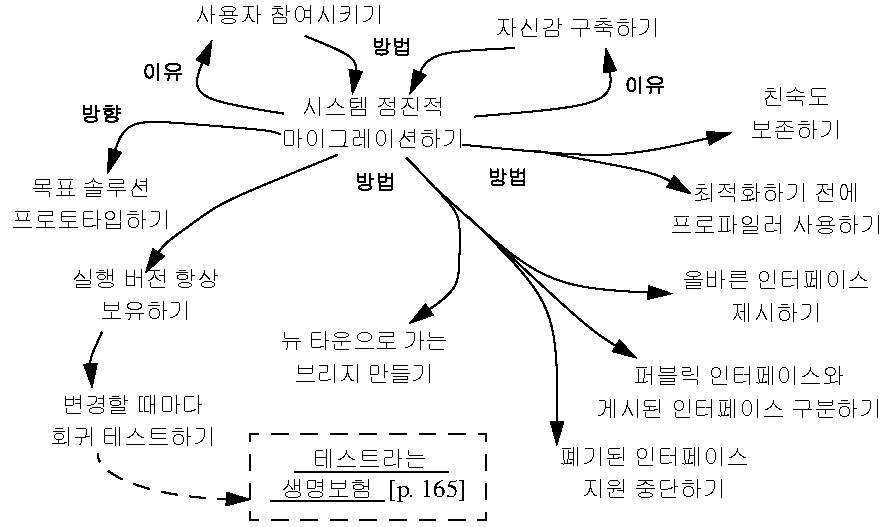
\includegraphics[width=\textwidth]{oldMigrationMap.pdf}
\caption{레거시 시스템을 마이그레이션하는 방법, 이유 및 대상}
\figlabel{MigrationMap}
\end{center}
\end{figure}

이 클러스터의 핵심 메시지는 \patref{시스템 점진적 마이그레이션하기}{MigrateSystemsIncrementally}이다. 그러나 이것은 말처럼 쉽지 않다. 그림 25에서 \patref{시스템 점진적 마이그레이션하기}{MigrateSystemsIncrementally}를 수행하려면 수많은 다른 패턴을 고려해야 한다는 것을 알 수 있다. 시스템 마이그레이션에 대한 방대한 문헌이 존재하기 때문에 이 주제를 자세히 다루지는 않겠다. 그러나 객체 지향 레거시 시스템을 리엔지니어링하는 데 가장 중요하다고 생각되는 패턴을 선택하고 주요 요점을 요약했다. 적절한 경우에 대해 독자는 추가 정보 출처를 찾을 수 있다.

이 클러스터의 중심 패턴은 \patref{시스템 점진적 마이그레이션}{MigrateSystemsIncrementally}이지만, 핵심 동기는 \patref{사용자 참여시키기}{InvolveTheUsers}와 \patref{자신감 구축하기}{BuildConfidence}에서 제공된다. 이 처음 세 가지 패턴은 리스크를 최소화하고 성공 확률을 높이기 위한 기본 패턴이다.

\begin{bulletlist}
\item \patref{사용자 참여시키기}{InvolveTheUsers}는 전체 리엔지니어링 프로세스에 사용자를 긴밀하게 참여시키고, 중간 결과물을 사용하게 하고, 강력한 지원을 제공함으로써 사용자가 새로운 시스템을 받아들일 가능성을 높인다. 단계별로 \patref{시스템 점진적 마이그레이션하기}{MigrateSystemsIncrementally}와 \patref{자신감 구축하기}{BuildConfidence}를 사용하면 더 쉽게 달성할 수 있다.

\item \patref{자신감 구축하기}{BuildConfidence}는 사용자에게 가치 있는 결과를 정기적으로 제공함으로써 회의론과 의심을 극복하는 데 도움이 된다. 

\item \patref{시스템 점진적 마이그레이션하기}{MigrateSystemsIncrementally}는 기존 시스템을 점진적이고 점진적으로 새 시스템으로 대체할 것을 권장한다. 그런 다음 진행하면서 새로운 결과를 통합할 수 있으므로 \patref{자신감 구축하기}{BuildConfidence} 및 \patref{사용자 참여시키기}{InvolveTheUsers}에 도움이 된다.
\end{bulletlist}

다음 사례도 준수하지 않으면 \patref{시스템 점진적 마이그레이션하기}{MigrateSystemsIncrementally}를 수행하기가 매우 어렵다.

\begin{bulletlist}
\item \patref{목표 솔루션 프로토타입하기}{PrototypeTheTargetSolution}을 사용하여 새 아키텍처와 새로운 기술적 리스크를 테스트한다. 이미 실행 중인 시스템이 있기 때문에 프로토타입이 필요 없다고 생각하기 쉽지만, 이는 거의 항상 실수이다.

\item \patref{실행 버전 항상 보유하기}{AlwaysHaveARunningVersion}는 변경 사항을 자주 통합하여 동기화 상태를 유지하는 데 도움이 된다.

\item \patref{변경할 때마다 회귀 테스트하기}{RegressionTestAfterEveryChange}는 실행 중이던 모든 것이 계속 실행되도록 함으로써 \patref{실행 버전 항상 보유하기}{AlwaysHaveARunningVersion}에 도움이 된다. 여기에는 \patpgref{진화 활성화를 위한 테스트 작성하기}{WriteTestsToEnableEvolution}가 전제되어 있다.
\end{bulletlist}

상황에 따라 \patref{시스템 점진적 마이그레이션하기}{MigrateSystemsIncrementally}에 도움이 될 수 있는 다양한 방법이 있다.

\begin{bulletlist}
\item \patref{뉴 타운으로 가는 브리지 만들기}{MakeABridgeToTheNewTown}는 (데이터) ``다리''의 은유를 도입하여 레거시 컴포넌트에서 대체 컴포넌트로 데이터를 점진적으로 마이그레이션하는 동시에 두 요소가 함께 실행될 수 있도록 한다. 모든 데이터가 전송되면 레거시 컴포넌트를 폐기할 수 있다.

\item \patref{올바른 인터페이스 제시하기}{PresentTheRightInterface}는 이전 기능을 래핑하여 실제로 원하는 추상화를 내보내 목표 시스템을 점진적으로 개발하는 데 도움이 된다.

\item \patref{퍼블릭 인터페이스와 게시된 인터페이스 구분하기}{DistinguishPublicFromPublishedInterface}는 리엔지니어링 팀 내에서 병렬 개발을 용이하게 하기 위해 안정적인 (퍼블릭) 인터페이스(public interface)와 불안정한 (게시된) 인터페이스(published interface)를 구분한다.

\item \patref{폐기된 인터페이스 지원 중단하기}{DeprecateObsoleteInterfaces}를 사용하면 클라이언트를 즉시 무효화하지 않고도 사용되지 않는 인터페이스를 정상적으로 폐기할 수 있다.
\end{bulletlist}

마지막으로, 다음 두 가지 방법은 급진적이지만 불필요한 변경을 피하는 데 도움이 될 수 있다.


\begin{bulletlist}
\item  \patref{친숙도 보존하기}{ConserveFamiliarity}는 사용자가 어색함을 느낄 수 있는 급격한 인터페이스 변경을 도입하지 않도록 경고한다.

\item \patpgref{최적화하기 전에 프로파일러 사용하기}{UseProfilerBeforeOptimizing}은 문제가 있음을 입증하고 문제의 원인을 정확히 파악하여 성능 문제를 고려하도록 한다.
\end{bulletlist}

%=================================================================
%:PATTERN -- {Involve the Users}
\pattern{사용자 참여시키기}{InvolveTheUsers}

\ind{고객과 관계맺기}\emph{(Engage Customers)로도 알려져 있다.} \cite{Copl95d}

\intent{모든 단계에서 사용자를 참여시켜 변경 사항의 수용을 극대화한다.}

\subsection*{문제}

사용자가 리엔지니어링된 시스템을 받아들일 것이라고 어떻게 확신할 수 있는가?

\emph{이 문제는 다음과 같은 이유로 어렵다.}

\begin{bulletlist}
\item 이전 시스템이 작동한다. 투박하지만 사용자들은 작동 방식을 알고 있고 문제를 해결하는 방법을 알고 있다.

\item 사람들은 자신의 삶을 더 편리하게 만들어 주지 않는 한 새로운 것을 배우는 것을 싫어한다.

\item 시스템 개선에 필요한 사항에 대한 사용자의 인식은 시스템이 발전함에 따라 변화하는 경향이 있다.

\item 사용자는 종이 위에만 있는 설계를 평가하는 것은 어려워 한다.

\item 사용할 준비가 되지 않은 새로운 시스템을 사용자가 좋아하게 만드는 것은 어렵다.
\end{bulletlist}

\emph{그러나 이 문제를 해결할 수 있는 이유는 다음과 같다.}

\begin{bulletlist}
\item 사용자는 자신의 요구가 진지하게 해결되고 있다고 판단되면 새로운 솔루션을 시도할 것이다.

\item 사용자는 유용한 정보를 제공하면 피드백을 줄 것이다.
\end{bulletlist}

\subsection*{해결}

사용자를 새로운 개발에 직접 참여시키고 새로운 시스템을 사용할 수 있도록 긴밀하게 지원하자.

\subsubsection*{단계}

사용자가 우선순위가 어디에 있는지 말할 수 있도록 하자. \patpgref{가장 가치 있는 것 먼저 하기}{MostValuableFirst}로 시작하자. 우선순위를 정기적으로 전달할 수 있는 작은 단계로 나누면 \patpgref{자신감 구축하기}{BuildConfidence}와 같이 사용할 수 있다.

사용자와 개발자 간의 접촉을 장려할 수 있는 환경을 조성하자. 물리적 위치가 중요하다.

정기적으로 중간 결과물을 전달하고 피드백을 받을 수 있는 간단한 절차를 마련하자. 초기 프로토타입은 특히 리스크가 큰 신기술이나 접근 방식을 평가하는 데 도움이 될 수 있다. 좋은 전략은 사용자가 새 시스템이 구축되는 대로 사용할 수 있도록 \patpgref{시스템 점진적 마이그레이션하기}{MigrateSystemsIncrementally}를 수행하는 것이다. 사용자가 느끼는 친숙도를 떨어 뜨리지 하기 위해 \patpgref{친숙도 보존하기}{ConserveFamiliarity}를 설정해야 한다.

\subsection*{트레이드오프}

\subsubsection*{장점}

\begin{bulletlist}
\item 요구사항이 지속적으로 검증되고 업데이트되므로 올바른 방향으로 나아갈 가능성이 높아진다.

\item 사용자가 유용한 결과를 얻고 있고 지원을 받고 있다고 느끼면 유용한 피드백을 제공하기 위해 더 많은 노력을 기울일 것이다.

\item 사용자가 프로젝트 전반에 걸쳐 참여하므로 프로젝트 후반에 특별한 교육 세션이 필요하지 않다.
\end{bulletlist}

\subsubsection*{단점}

\begin{bulletlist}
\item 개발자는 사용자를 지원하는 것이 시스템 리엔지니어링 작업에 방해가 된다고 느낄 수 있다.

\index{유든, 에드워드}
\item 사용자 참여가 성공하면 기대치가 높아지고 팀에 추가적인 압박이 가해진다. 예를 들어, 유든은 프로토타입은 기대치를 지나치게 높일 수 있으며 아직 작동하지 않는 부분을 항상 명확히 해야 한다고 이야기 한다 \cite{Your97a}.
\end{bulletlist}

\subsubsection*{어려움}

\begin{bulletlist}
\item 결과를 보여 줄 수 있기 전까지는 사용자를 참여를 시작하기 어려울 수 있다.

\item 모든 사용자를 참여시킬 수는 없으며, 포함되지 않은 사용자는 소외감을 느낄 수 있다.
\end{bulletlist}

\subsection*{근거}

실제 고객의 요구 사항을 다루려면 피드백 루프가 필요하다. 사용자를 참여시키고 지원함으로써 이러한 피드백 루프가 활성화 되도록 할 수 있다.

\index{코플리언, 제임스}
\emph{```제품 품질 유지(maintaining product quality)'가 여기서 해결해야 할 문제가 아니라는 점에 유의하자. 제품 품질은 고객 만족의 한 요소일 뿐이다.''}라고 코플리언은 지적했다. \cite{Copl95d}

\subsection*{관련 패턴}

이 클러스터의 거의 모든 패턴은 \patref{사용자 참여시키기}{InvolveTheUsers}를 지원한다. \patref{시스템 점진적 마이그레이션 하기}{MigrateSystemsIncrementally}를 통해 사용자가 리엔지니어링 중인 시스템을 함께 작업하도록 하여 \patref{자신감 구축하기}{BuildConfidence}를 구현한다.

\ind{계획 게임}\emph{(Planning Game)} \cite{Beck01a}는 반복적으로 스토리를 파악하고, 비용을 추산하고, 출시할 스토리를 제품에 적용함으로써 \patref{사용자 참여시키기}{InvolveTheUsers}를 구현하는 효과적인 기법이다.

%=================================================================
%:PATTERN -- {Build Confidence}
\pattern{자신감 구축하기}{BuildConfidence}

\intent{규칙적으로 성과를 보여줌으로써 전반적인 성공 가능성을 높인다.}

\subsection*{문제}

모든 종류의 소프트웨어 프로젝트에 대해 고객과 팀원이 종종 갖는 높은 수준의 회의감(skepticism)을 어떻게 극복할 수 있는가?

\emph{이 문제는 다음과 같은 이유로 어렵다.}

\begin{bulletlist}
\item 요구 사항을 충족하고 제시간에 완료되며 예산 범위 내에서 진행되는 소프트웨어 프로젝트는 거의 없다. 대부분의 프로젝트에 수반되는 회의주의는 쉽게 패배주의(defeatism)로 이어질 수 있으며, 프로젝트는 자기 충족적 예언처럼 실패할 수 있다.

\item 사용자가 진정으로 원하거나 필요로 하는 것을 거의 얻지 못한다.

\item 레거시 시스템을 실제로 잘 유지할 수 있다고 사용자나 팀원들을 설득하기 어려울 수 있다.
\end{bulletlist}

\emph{그러나 이 문제를 해결할 수 있는 이유는 다음과 같다.}

\begin{bulletlist}
\item 모든 문제를 한 번에 해결할 필요는 없습니다.
\end{bulletlist}

\subsection*{해결}

가능한 한 빨리 긍정적인 결과를 보여줌으로써 긍정적인 분위기를 조성하고, 정기적으로 계속 그렇게 하자.

\subsubsection*{단계}

짧은 간격을 두고 새로운 결과를 전달하자. 각 단계에서 실질적인 가치를 보여줄 수 있는 최소한의 결과가 무엇인지 사용자와 함께 합의하자.

\subsection*{트레이드오프}

\subsubsection*{장점}

\begin{bulletlist}
\item 사용자와 개발자 모두 실제 진행 상황을 측정할 수 있다.

\item 작은 단계의 비용을 더 쉽게 추정할 수 있다.
\end{bulletlist}

\subsubsection*{단점}

\begin{bulletlist}
\item 사용자와 자주 동기화하는 데 시간이 걸린다.

\item 사용자는 새 시스템을 이전 시스템과 함께 사용하는 데 필요한 추가 작업을 거부할 수 있다.

\item 프로젝트 초기에 좋은 결과를 보여 주는 데 성공하면 기대치가 너무 높아질 수 있다.
\end{bulletlist}

\subsubsection*{어려움}

\begin{bulletlist}
\item 일부 요구 사항은 특히 시스템의 아키텍처 변경을 수반하는 경우 작은 단계로 나누기 어려울 수 있다.

\item 리엔지니어링 팀은 가장 중요한 정보 소스 중 하나인 원래 시스템의 개발자를 소외시키지 않도록 주의해야 한다.

\item 사용자를 설득하는 것만으로는 충분하지 않으며 경영진의 동의를 얻는 데도 신경을 써야 한다. 작은 단계로 경영진을 설득하기는 어렵다. 정기적으로 대규모 데모를 계획하자.
\end{bulletlist}

\subsection*{근거}

작은 단계를 밟아나가면 개별 단계가 실패할 리스크를 줄일 수 있다. 긍정적인 결과를 자주 얻으면 자신감을 키우는 데 도움이 된다. 같은 맥락에서 \ind{익스트림 프로그래밍}(Extreme Programming)은 \ind{소규모 릴리즈}(Small Releases)를 지지한다. \cite{Beck00a}. 부정적인 결과라도 진행 상황을 모니터링하고 상황을 더 잘 이해하는 데 도움이 되므로 자신감을 키우는 데 도움이 된다.

\subsection*{관련 패턴}

\patref{목표 솔루션 프로토타입 만들기}{PrototypeTheTargetSolution}와 \patref{뉴 타운으로 가는 브리지 만들기}{MakeABridgeToTheNewTown}를 사용하면 작은 단계로 결과를 쉽게 보여줄 수 있다. 

\patref{사용자 참여시키기}{InvolveTheUsers}를 사용하면 \patref{자신감 구축하기}{BuildConfidence}를 더 쉽게 수행할 수 있다. 

%=================================================================
%:PATTERN -- {Migrate Systems Incrementally}
\pattern{시스템 점진적 마이그레이션하기}{MigrateSystemsIncrementally}

\ind{치킨 리틀}(Chicken Little)로도 \emph{알려져 있다}. \cite{Brod95a}

\intent{기능을 빈번한 증분 개념으로 배포함으로써 빅뱅 리엔지니어링의 복잡성과 리스크를 피하자.}

\subsection*{문제}

새 시스템 배포는 언제 계획해야 하는가?

\emph{이 문제는 다음과 같은 이유로 어렵다.}

\begin{bulletlist}
\item 프로젝트는 ``빅뱅'' 요구 사항 사양을 미리 작성하여 대규모로 계획하고 자금을 지원하는 경우가 많다.

\item 실제 요구사항은 뒤늦게야 명확해지는 경우가 많다. 특히 처음부터 완벽하게 작동하지 않는다면 사용자는 익숙한 것과 근본적으로 다른 새로운 시스템 사용을 거부할 것이다.

\item 새 시스템을 배포하는 데 시간이 오래 걸릴수록 사용자 피드백을 받기 위해 더 오래 기다려야 한다.

\item 불완전한 시스템을 배포할 수 없다. 사용자는 불완전한 솔루션에 시간을 낭비하고 싶어하지 않는다.
\end{bulletlist}

\emph{그러나 이 문제를 해결할 수 있는 이유는 다음과 같다.}

\begin{bulletlist}
\item 확장 및 수정할 수 있는 동작하는 시스템이 있다.
\end{bulletlist}

\subsection*{해결}

가능한 한 빨리 레거시 시스템의 첫 번째 \emph{업데이트(update)}를 배포하고 대상 시스템으로 점진적으로 마이그레이션하자.

\subsubsection*{단계}

\begin{bulletlist}
\item 레거시 시스템을 여러 부분으로 분해한다.

\item 한 번에 하나씩 처리할 부분을 선택한다.

\item 해당 부분과 해당 부분에 의존하는 부분에 대한 테스트를 수행한다.

\item 레거시 컴포넌트를 래핑, 리엔지니어링 또는 교체하기 위한 적절한 조치를 취한다.

\item 업데이트된 컴포넌트를 배포하고 피드백을 받는다.

\item 반복한다.
\end{bulletlist}

\subsection*{트레이드오프}

\subsubsection*{장점}

\begin{bulletlist}
\item 사용자 피드백을 조기에 받고 \patref{자신감 구축하기}{BuildConfidence}를 수행한다.

\item 문제가 발생하면 즉시 알 수 있다.

\item 사용자는 새 시스템이 구축되는 동안 학습한다.

\item 시스템이 항상 배포된다.

\item 시스템은 항상 테스트 중이므로 테스트를 건너뛸 수 없다.
\end{bulletlist}

\subsubsection*{단점}

\begin{bulletlist}
\item 시스템을 변경하는 동안 시스템을 계속 실행하려면 더 많은 노력을 기울어야 한다.
\end{bulletlist}

\subsubsection*{어려움}

\begin{bulletlist}
\item 새로운 아키텍처로 마이그레이션하는 것이 어려울 수 있다. 새 아키텍처를 적용하기 위해 \patref{목표 솔루션 프로토타입하기}{PrototypeTheTargetSolution}를 사용할 수 있다, 그리고 기본 구성 요소를 마이그레이션하는 동안 레거시 인터페이스를 숨기려면 \patref{올바른 인터페이스 제시하기}{PresentTheRightInterface}를 이전 시스템에 적용할 수 있다.

\item 실행 중인 시스템을 변경하는 것은 리스크가 크다. 반드시 \patref{변경할 때마다 회귀 테스트하기}{RegressionTestAfterEveryChange}를 수행하자. 
\end{bulletlist}

\subsection*{근거}

실행 중인 시스템에서 최고의 사용자 피드백을 얻을 수 있다. 사용자는 매일 사용하는 시스템에서 피드백을 제공하는 더 많은 동기를 얻고 참여할 수 있다.

\subsection*{알려진 용도}

\emphind{Migrating Legacy Systems} \cite{Brod95a}에서는 이 패턴을 '\ind{치킨 리틀}(Chiceken Little)'이라는 이름으로 소개한다(점진적으로 마이그레이션한다는 것은 '치킨 리틀 단계를 밟는다'는 뜻이다). 이 책에서는 점진적 마이그레이션을 위한 전략과 기법에 대해 자세히 설명한다.

\subsection*{관련 패턴}

\patpgref{가장 가치 있는 것 먼저 하기}{MostValuableFirst}를 적용하여 먼저 작업할 레거시 컴포넌트를 선택한다. 아키텍처 무결성을 유지하기 위해 \patpgref{내비게이터 지정하기}{AppointANavigator}를 적용한다. 

마이그레이션할 때 \patpgref{진화 활성화를 위한 테스트 작성하기}{WriteTestsToEnableEvolution}, \patpgref{기본 테스트를 증가시키기}{GrowYourTestBaseIncrementally}를 실행하자. 레거시 컴포넌트를 리엔지니어링하거나 교체할 때 항상 테스트를 다시 작성할 필요가 없도록 \patpgref{구현이 아닌 인터페이스 테스트하기}{TestTheInterfaceNotTheImplementation}을 사용하자. \patref{변경할 때마다 회귀 테스트하기}{RegressionTestAfterEveryChange}를 사용하면 \patpgref{실행 버전 항상 보유하기}{AlwaysHaveARunningVersion}을 사용할 수 있다.

리엔지니어링하거나 교체할 의도가 없는 레거시 컴포넌트에 대해서는 \patref{올바른 인터페이스 제시하기}{PresentTheRightInterface}를 적용하는 것이 좋다.

교체하려는 레거시 컴포넌트에서 데이터를 마이그레이션해야 하는 경우 \patpgref{뉴 타운으로 가는 브리지 만들기}{MakeABridgeToTheNewTown}을 적용할 수 있다.

%=================================================================
%:PATTERN -- {Prototype the Target Solution}
\pattern{목표 솔루션 프로토타입하기}{PrototypeTheTargetSolution}

\intent{프로토타입을 만들어 새 대상 솔루션으로 마이그레이션할 리스크를 평가한다.}

\subsection*{문제}

새 목표 시스템에 대한 아이디어가 효과가 있는지 어떻게 알 수 있는가?

\emph{이 문제는 다음과 같은 이유로 어렵다.}

\begin{bulletlist}
\item 작동 중인 시스템을 급격하게 변경하는 것은 리스크가 크다.

\item 설계 변경이 기존 기능에 어떤 영향을 미칠지 예측하기 어려울 수 있다.

\item 작동하는 솔루션이 테스트되지 않은 솔루션보다 더 신뢰할 수 있다.
\end{bulletlist}

\emph{그러나 이 문제를 해결할 수 있는 이유는 다음과 같다.}

\begin{bulletlist}
\item 새로운 아이디어를 테스트하기 위해 레거시 시스템 전체를 리엔지니어링할 필요는 없다.
\end{bulletlist}

\subsection*{해결}

새로운 개념을 위해 개발한 프로토타입을 가지고 새롭고 창발하는 요구 사항에 대해 평가하자.

\subsubsection*{단계}

\begin{bulletlist}
\item 리엔지니어링 프로젝트의 가장 큰 기술적 르시크를 파악하자. 일반적으로 다음과 같은 우려 사항이 있다.

\begin{bulletlist}
\item 새로운 시스템 아키텍처의 선택
\item 레거시 데이터의 새 시스템으로의 마이그레이션
\item 새로운 기술 또는 플랫폼을 통한 적절한 성능 또는 성능 향상(예: 특정 트랜잭션 처리량을 달성할 수 있음을 입증)
\end{bulletlist}

\index{버려질 프로토타입}
\index{탐색용 프로토타입}
\index{진화적 프로토타입}
\item 기술 옵션의 실현 가능성을 순수하게 평가하기 위한 탐색용 프로토타입(exploratory prototype) 즉, 버려질 프로토타입(throwaway prototype)을 구현할지 아니면 최종적으로 새로운 목표 시스템으로 진화할 진화적 프로토타입(evolutionary prototype)을 구현할지 결정합니다.

\begin{bulletlist}
\item 탐색용 프로토타입(exploratory prototype)은 매우 정확한 질문에 답할 수 있도록 설계되어야 한다. 이러한 질문은 새 플랫폼이 레거시 시스템에서 설정한 성능 제약을 충족할 수 있는지와 같은 순전히 기술적인 질문일 수도 있고, 사용자의 참여와 평가가 필요한 사용성 질문일 수도 있다. 탐색용 프로토타입은 (이 프로토타입이 제공하는 답변이 새 시스템에 영향을 미치기는 하지만) 다른 문제나 질문을 해결하기 위해 설계될 필요가 없으며 마이그레이션헐 시스템의 일부가 아니다.

\item 반면에 진화형 프로토타입(evolutionary prototype)은 궁극적으로 레거시 구성 요소를 대체하기 위한 것이므로 목표 아키텍처를 반영해야 한다. 새로운 아키텍처는 레거시 서비스를 가장 적절하게 지원할 뿐만 아니라 레거시 솔루션의 유용성을 제한하는 장애물도 극복한다. 프로토타입은 이러한 리스크에 먼저 대응할 수 있도록 설계되어야 한다.
\end{bulletlist}
\end{bulletlist}

\subsection*{트레이드오프}

\subsubsection*{장점}

\begin{bulletlist}
\item 레거시 시스템의 모든 기능을 구현할 필요가 없으므로 프로토타입을 빠르게 구축할 수 있다.

\item 프로토타입을 실행하기 위해 레거시 시스템의 일부를 해킹할 수 있다.

\item 목표 시스템에 대한 아이디어가 타당하다면 빠르게 학습할 수 있다.
\end{bulletlist}

\subsubsection*{단점}

\begin{bulletlist}
\item 사용자는 버려질 프로토타입을 평가하는 데 많은 시간을 할애할 동기가 높지 않을 수 있다.

\item 버려질 프로토타입을 버리지 않고 계속 개발하고 싶은 유혹을 받을 수 있다.
\end{bulletlist}

\subsubsection*{어려움}

\begin{bulletlist}
\item 결국 이미 실행 중인 시스템이 있기 때문에, 자신이나 고객에게 프로토타입의 필요성을 설득하기 어려울 수 있다.

\item 진화적 프로토타입을 완성하는 데 너무 많은 시간이 걸릴 수 있다. 레거시 컴포넌트에 \patref{올바른 인터페이스 제시하기}{PresentTheRightInterface}를 적용하여 프로토타입에 레거시 서비스를 위한 좋은 인터페이스를 제공하는 것을 고려하자. 
\end{bulletlist}

\subsection*{근거}

\index{브룩스, 프레드릭}
프로토타입은 특정 기술적 접근 방식이 올바른지 아닌지를 빠르게 알려줄 수 있다. \emph{맨먼스 미신(The Mythical Man-Month)}의 브룩스 \cite{Broo75a}는 처음부터 제대로 만들기는 어렵기 때문에 '버릴 것은 버려라'라고 조언한다.
\index{러브, 톰}
\index{푸트, 브라이언}
\index{요더, 조셉}
러브는 여기서 한 걸음 더 나아가 객체 지향 시스템의 경우 ``버릴 것을 각오하고 두 번 구현해야 한다(write two to throw away)''고 경고한다\cite{Love93a}. 푸트와 요더는 무엇보다도 \ind{버릴 임시 코드(Throwaway Code)}가 도메인 요구 사항을 명확히 하는 가장 좋은 방법이라고 주장하지만, 프로토타입이 ``\ind{큰 진흙 뭉치(Big Ball of Mud)}''로 발전할 리스크가 있다고 경고하기도 한다\cite{Foot00a}.

\subsection*{관련 패턴}

\patref{뉴타운으로 가는 다리 만들기}{MakeABridgeToTheNewTown}을 적용하여 레거시 데이터를 진화하는 프로토타입으로 마이그레이션하는 것을 고려할 수 있다.

%=================================================================
%:PATTERN -- {Always Have a Running Version}
\pattern{실행 버전 항상 보유하기}{AlwaysHaveARunningVersion}


\intent{주기적으로 시스템을 리빌드하여 변경 사항에 대한 신뢰도를 높인다.}

\subsection*{문제}

올바른 길을 가고 있다고 어떻게 고객을 확신시킬 수 있는가?

\emph{이 문제는 다음과 같은 이유로 어렵다.}

\begin{bulletlist}
\item 개발 중인 소프트웨어 시스템을 데모하거나 사용자와 문제를 논의하기 어려울 수 있다. 시스템의 안정적으로 실행되는 버전이 없는 경우가 많기 때문이다.

\item 여러 버전의 시스템에서 변경 사항을 통합하는 작업은 느리고 번거로울 수 있다.
\end{bulletlist}

\emph{그러나 이 문제를 해결할 수 있는 이유는 다음과 같다.}

\begin{bulletlist}
\item 시스템 통합을 위해 컴포넌트 ``구현 완료''를 기다릴 필요가 없다.
\end{bulletlist}

\subsection*{해결}

매일 새로운 변경 사항과 개발 사항을 통합하는 규칙을 확립하자.

\subsubsection*{단계}

\begin{bulletlist}
\item 버전 관리 및 형상 관리(configuration management) 시스템을 마련하자.

\item 작업 중인 부분에 대한 회귀 테스트가 마련되어 있는지 확인하자.

\item 시스템 컴포넌트를 체크 아웃하고 다시 체크인하는 짧은 트랜잭션 규율을 마련하자. 변경 사항이 실행 중인 시스템에 통합될 수 있도록 가능한 한 짧게 반복(iteration)을 계획하자.
\end{bulletlist}

\subsection*{트레이드오프}

\subsubsection*{장점}

\begin{bulletlist}
\item 항상 데모할 수 있는 작동하는 버전이 있다.

\item 회귀 테스트를 실행하기 위해 항상 작동하는 버전을 사용할 수 있다.

\item 변경 사항을 빠르게 검증할 수 있어 \patref{자신감 구축하기}{BuildConfidence}에 도움이 된다.
\end{bulletlist}

\subsubsection*{단점}

\begin{bulletlist}
\item 변경 사항을 지속적으로 통합해야 한다.
\end{bulletlist}

\subsubsection*{어려움}

\begin{bulletlist}
\item 대규모 시스템의 경우 빌드 시간이 매우 길어질 수 있다. 빌드 시간을 단축하려면 먼저 시스템을 재설계해야 할 수 있다.

\item 일부 종류의 대규모 수정 사항을 개별적으로 통합할 수 있는 의미 있는 업데이트로 나누기가 어려울 수 있다.
\end{bulletlist}

\subsection*{근거}

많은 실무자들은 리스크가 크고 고통스러운 빅뱅 통합을 피하기 위한 방법으로 지속적 통합 프로세스를 지지한다 \cite{Booc94a}.

\subsection*{관련 패턴}

\patref{변경할 때마다 회귀 테스트하기}{RegressionTestAfterEveryChange}는 통합 중에 결함이 발생할 리스크를 최소화한다.

\ind{지속적 통합(Continuous Integration)} \cite{Booc94a} \cite{Beck00a}는 \patref{실행 버전 항상 보유하기}{AlwaysHaveARunningVersion}에 대한 입증된 방법이다.

%=================================================================
%:PATTERN -- {Regression Test After Every Change}
\pattern{변경할 때마다 회귀 테스트하기}{RegressionTestAfterEveryChange}


\intent{이전에도 효과가 있었던 것이 여전히 효과가 있는지 확인하여 신뢰를 구축한다.}

\subsection*{문제}

마지막으로 변경한 내용이 시스템을 손상시키지 않는다는 것을 어떻게 확신할 수 있는가?

\emph{이 문제는 다음과 같은 이유로 어렵다.}

\begin{bulletlist}
\item 복잡한 시스템에서는 작은 변경이 예상치 못한 부작용을 초래할 수 있습니다. 무해해 보이는 변경이 즉시 발견되지 않고 무언가를 망가뜨릴 수 있다.
\end{bulletlist}

\emph{그러나 이 문제를 해결할 수 있는 이유는 다음과 같다.}

\begin{bulletlist}
\item 시스템이 어떻게 동작해야 하는지 표현하는 테스트 스위트(test suite)를 작성했다.
\end{bulletlist}

\subsection*{해결}

안정적인 상태에 도달했다고 생각될 때마다 회귀 테스트 스위트를 실행하자.

\subsection*{트레이드오프}

\subsubsection*{장점}

\begin{bulletlist}
\item \patref{실행 버전 항상 보유하기}{AlwaysHaveARunningVersion}가 더 쉽다.

\item 진행하면서 \patref{자신감 구축하기}{BuildConfidence}가 더 쉽다.
\end{bulletlist}

\subsubsection*{단점}

\begin{bulletlist}
\item 테스트를 끊임없이 작성해야 한다. 
\end{bulletlist}

\subsubsection*{어려움}

\begin{bulletlist}
\item 레거시 시스템에 적절한 회귀 테스트가 정의되어 있지 않을 수 있다. 시스템이 진화하도록 하려면 \patpgref{기본 테스트를 증가시키기}{GrowYourTestBaseIncrementally}를 사용해야 한다.

\item 테스트는 결함이 있다는 것만 보여줄 수 있고 결함이 없다는 것은 보여주지 못한다. 망가져 있는 부분을 정확하게 테스트하지 못했을 수 있다.

\item 테스트를 실행하는 데 시간이 많이 걸릴 수 있으므로 변경 사항으로 인해 영향을 받을 수 있다고 생각되는 테스트만 실행하는 것이 좋다. 변경 사항에 대한 ``에드혹'' 테스트를 피하기 위해 테스트를 분류하되, 모든 테스트를 적어도 하루에 한 번씩 실행하자.
\end{bulletlist}

\subsection*{근거}

회귀 테스트는 이전에 실행된 테스트가 여전히 동작되고 있음을 알려준다. 발견한 결함과 새로운 기능에 대한 테스트를 지속적으로 구축하면 재사용 가능한 테스트 기반을 확보하게 되어 변경 사항이 건전하다는 확신을 갖게 되고 문제를 조기에 발견하는 데 도움이 된다.

\index{데이비스, 앨런}
데이비스는  ``\patref{변경할 때마다 회귀 테스트하기}{RegressionTestAfterEveryChange}''를 표준 소프트웨어 개발 실천법으로 \cite{Davi95a}를 권장한다.

\subsection*{관련 패턴}

이미 \patpgref{진화 활성화를 위한 테스트 작성하기}{진화 활성화를 위한 테스트 작성하기}를 시작했어야 한다. 

\index{테스트 주도 개발(Test-Driven development)} \ind{익스트림 프로그래밍(Extreme Programming)}의 일반적인 실천법은 새로운 기능을 구현하기 \cite{Jeff01a} \emph{전에} 테스트를 작성하는 것이다. 리엔지니어링의 맥락에서는 변경을 하기 전에 실패하고 변경이 올바르게 구현되면 통과하는 테스트를 작성하는 것을 고려해야 한다. (안타깝게도 변경이 올바른 \emph{경우에만} 성공하는 테스트를 설계하는 것은 일반적으로 불가능하다!).

회귀 테스트는 \patpgref{지속적인 문제 재테스트하기}{RetestPersistentProblems}에 도움이 된다.

%=================================================================
%:PATTERN -- {Make a Bridge to the New Town}
\pattern{뉴 타운으로 가는 브리지 만들기}{MakeABridgeToTheNewTown}

\ind{뉴 타운으로 가는 다리(Bridge to the New Town)} \cite{Kell00a}, \ind{데이터 유지 --- 코드 전달(Keep the Data --- Toss the Code)} \cite{Brod95a}로도 알려져 있다.

\intent{브릿지를 사이에 두고 새 시스템을 병렬로 실행하여 레거시 시스템에서 데이터를 마이그레이션한다.}

\subsection*{문제}

두 시스템이 병렬로 실행되는 동안 레거시 시스템에서 대체 시스템으로 데이터를 점진적으로 마이그레이션하려면 어떻게 해야 하는가?

\emph{이 문제는 다음과 같은 이유로 어렵다.}

\begin{bulletlist}
\item 레거시 시스템의 일부 컴포넌트는 수리가 불가능하여 교체해야 한다.

\item 중요 컴포넌트의 갑작스러운 교체(Big-bang replacement)는 매우 리스크가 크다.

\item 레거시 컴포넌트에 의해 조작되는 \emph{데이터}는 마이그레이션하는 동안 사용 가능한 상태로 유지되어야 한다.
\end{bulletlist}

\emph{그러나 이 문제를 해결할 수 있는 이유는 다음과 같다.}

\begin{bulletlist}
\item 동작하는 레거시 시스템이 있다.
\end{bulletlist}

\subsection*{해결}

\begin{figure}
\begin{center}
\includegraphics[width=0.75\textwidth]{MigrationBridge}
\caption{브리지(bridge)를 사용하면 데이터를 새 시스템으로 투명하게 전송할 수 있다.}
\figlabel{MigrationBridge}
\end{center}
\end{figure}

새 컴포넌트가 레거시 시스템에서 데이터를 가져 올 준비가 되면 레거시 시스템에서 교체할 시스템으로 데이터를 점진적으로 전송하는 (데이터) 브리지를 만들자.

\subsubsection*{단계}

\begin{bulletlist}
\item 동일한 논리 데이터 엔티티를 처리하는 레거시 시스템과 교체 시스템의 컴포넌트를 구별한다.

\item 데이터가 아직 마이그레이션되지 않은 경우 새 컴포넌트에서 레거시 데이터 소스로 \emph{읽기(read)} 요청을 리디렉션하는 ``\ind{데이터 브리지}(data bridge)''를 구현한다. 브리지는 필요한 모든 데이터 변환을 담당한다. 새 컴포넌트는 브리지를 인식해서는 안 된다.

\item 레거시 컴포넌트를 조정하여 새 데이터가 최신 상태로 유지되도록 \emph{쓰기(write)} 요청을 새 컴포넌트로 리디렉션한다.

\item 모든 데이터를 옮기면 브리지와 레거시 컴포넌트를 제거한다.
\end{bulletlist}

\subsection*{트레이드오프}

\subsubsection*{장점}

\begin{bulletlist}
\item 모든 레거시 데이터를 마이그레이션하지 않고 새 시스템 사용을 시작할 수 있다.
\end{bulletlist}

\subsubsection*{단점}

\begin{bulletlist}
\item 레거시 데이터와 새 데이터 사이에 간단한 매핑이 없는 경우 데이터 브리지를 올바르게 구현하기가 까다로울 수 있다.

\item 일부 데이터가 옮겨지면 되돌리기가 어려울 수 있다.

\item 데이터 브리지는 성능 오버헤드를 추가한다. 이는 허용될 수도 있고 허용되지 않을 수도 있다.
\end{bulletlist}

\subsubsection*{어려움}

\begin{bulletlist}
\item \emph{``단계별 마이그레이션 방식(Stepwise migration scheme)은 대규모의 레이어드 비즈니스 시스템에서 매우 효과적인 것으로 입증되었다. 체크인/체크아웃 지속성이 있고 결합도가 높고 매우 촘촘하게 짜여진 오브젝트 망이 있는 CAD 애플리케이션에서는 일반적이지 않다.''} \cite{Kell00a}
\end{bulletlist}

\subsection*{알려진 용도}

\index{브로디, 마이클}
\index{스톤브레이커, 마이클}
브로디와 스톤브레이커는\emph{레거시 시스템 마이그레이션(Migrating Legacy Systems)}에서 데이터 브리지 및 게이트웨이 사용에 대해 훨씬 더 자세히 설명한다. \cite{Brod95a}. 

\index{켈러, 울프강}
켈러는 ``뉴 타운으로 가는 브리지(The Bridge to the New Town)'' \cite{Kell00a}에서 레거시 데이터 마이그레이션의 기술적 문제에 더 중점을 두고 있으며, 이 패턴이 성공적으로 적용된 수많은 사례를 지적한다.

이 패턴에는 레거시 시스템 전체를 교체할 것인지, 아니면 컴포넌트 하나만 교체할 것인지, 그리고 사용자가 두 시스템에 동시에 액세스할 수 있어야 하는지 여부에 따라 다양한 변형이 가능하다.

\subsection*{근거}

이전 시스템과 새 시스템 간의 브리지를 사용하면 새 시스템이 완성되기 전에 사용자가 새 시스템의 기능을 사용할 수 있도록 할 수 있다. 브리지는 두 시스템을 서로 분리하여 레거시 시스템의 영향을 받지 않고 새로운 아키텍처 비전에 따라 새 시스템을 개발할 수 있도록 한다.

\subsection*{관련 패턴}

브리지는 \patref{시스템 점진적 마이그레이션하기}{MigrateSystemsIncrementally}를 지원하여 \patref{자신감 구축하기}{BuildConfidence}를 지원한다.

%=================================================================
%:PATTERN -- {Present the Right Interface}
\pattern{올바른 인터페이스 제시하기}{PresentTheRightInterface}

\ind{시맨틱 래퍼(Semantic Wrapper)} \cite{Ocal00a}, \ind{양탄자 밑으로 쓸어 넣기(Sweeping it Under the Rug)} \cite{Foot00a}로도 알려져 있다.

\intent{기존 구현에 반영되어 있지 않더라도 올바른 추상화를 드러나도록 레거시 시스템을 래핑한다.}

\subsection*{문제}

마이그레이션 프로세스 중에 새 목표 시스템이 레거시 서비스를 어떻게 액세스해야 하는가?

\emph{이 문제는 다음과 같은 이유로 어렵다.}

\begin{bulletlist}
\item 목표 시스템 구현이 아직 완료되지 않았으므로 마이그레이션하는 동안 레거시 서비스에 의존해야 한다. 

\item 레거시 시스템이 목표 시스템에 필요한 인터페이스를 제공하지 않는다.

\item 레거시 컴포넌트 측면에서 새 컴포넌트를 구현하면 목표 시스템이 레거시 아키텍처 및 디자인에 대해 편향이 발생한다.
\end{bulletlist}

\emph{그러나 이 문제를 해결할 수 있는 이유는 다음과 같다.}

\begin{bulletlist}
\item 레거시 서비스에 직접 액세스할 필요가 없다.
\end{bulletlist}

\subsection*{해결}

새 시스템에 포함할 추상화를 찾아네고 기존 소프트웨어를 래핑하여 새 추상화를 에뮬레이트한다.

\subsubsection*{힌트}

예를 들어 객체 지향 시스템 내에서 사용되는 절차적 그래픽 라이브러리를 생각해 보자. 이 라이브러리를 객체 지향 방식으로 다시 구현하려면 너무 많은 비용과 시간이 필요하다. 유틸리티 클래스(즉, 정적 메서드는 있지만 인스턴스가 없는 클래스)로 래핑하는 것이 더 쉽겠지만, 진정한 객체 지향 인터페이스를 제공하지만 기본 절차적 추상화를 사용하여 구현되는 약간 두꺼운 래퍼를 작성하는 것이 더 현명할 것이다. 이렇게 하면 새로운 시스템이 레거시 추상화에 의해 오염되지 않는다. 

\subsection*{트레이드오프}

\subsubsection*{장점}

\begin{bulletlist}
\item 처음부터 적절한 추상화를 사용할 수 있다면 목표 시스템을 레거시 서비스에서 떼어내기가 더 쉬워진다.

\item 레거시 설계가 새 대상에 악영향을 미칠 리스크를 줄일 수 있다.
\end{bulletlist}

\subsubsection*{단점}

\begin{bulletlist}
\item 새 인터페이스가 안정적이지 않을 수 있으므로 개발자가 사용을 꺼릴 수 있다.
\end{bulletlist}

\subsubsection*{어려움}

\begin{bulletlist}
\item 절차적 추상화를 단순히 유틸리티 클래스로 포장하고 싶은 유혹을 뿌리치기가 어려울 수 있다.
\end{bulletlist}

\subsection*{알려진 용도}

\index{오캘러한, 앨런}
앨런 오캘러한 \cite{Ocal00a}은 대규모 비즈니스 크리티컬 레거시 시스템을 객체 지향 및 컴포넌트 기반 기술로 마이그레이션하는 \ind{ADAPTOR 패턴}의 맥락에서 이 패턴을 ``\ind{시맨틱 래퍼}(Semantic Wrapper)''로 간략하게 제시한다. 

\subsection*{근거}

\patref{올바른 인터페이스 제시하기}{PresentTheRightInterface}는 레거시 설계의 관점에서 생각하지 않고 대체 접근 방식을 더 쉽게 고려할 수 있도록 해준다.

\subsection*{관련 패턴}

\patref{올바른 인터페이스 제시하기}{PresentTheRightInterface}는 둘 다 래퍼를 구현 기법으로 사용하기 때문에 표면적으로는 \patpgref{Adapter}{Adapter}와 비슷하다. 그러나 \patref{Adapter}{Adapter}는 호환되지 않는 인터페이스를 클라이언트가 기대하는 다른 인터페이스에 맞게 조정한다. 반면 \patref{올바른 인터페이스 제시하기}{PresentTheRightInterface}는 레거시 컴포넌트에 더 적합한 새 인터페이스를 소개한다. 

반드시 \patref{폐기된 인터페이스 지원 중단하기}{DeprecateObsoleteInterfaces}를 사용하자. 

\patref{올바른 인터페이스 제시하기}{PresentTheRightInterface}로 구현된 새 인터페이스가 안정적이지 않은 경우 \patref{공개 인터페이스와 게시된 인터페이스 구분하기}{DistinguishPublicFromPublishedInterface}를 사용해야 한다.

%=================================================================
%:PATTERN -- {Distinguish Public from Published Interface}
\pattern{퍼블릭 인터페이스와 게시된 인터페이스 구분하기}{DistinguishPublicFromPublishedInterface}

\ind{게시된 인터페이스}(Published Interface) \cite{Ocal00a}로도 알려져 있다.

\intent{불안정한 ``게시된 인터페이스(published interface)''와 안정적인 ``퍼블릭 인터페이스(published interface)''를 구분하여 병렬 개발을 용이하게 한다.}

\subsection*{문제}

새 인터페이스가 아직 개발 중인 동안 레거시 인터페이스에서 새 목표 인터페이스로 마이그레이션하려면 어떻게 해야 하는가?

\emph{이 문제는 다음과 같은 이유로 어렵다.}

\begin{bulletlist}
\item 가능한 한 빨리 새 목표 시스템으로 마이그레이션을 활성화하려고 한다.

\item 새 대상 컴포넌트의 인터페이스를 너무 일찍 고정하고 싶지 않다.

\item 널리 사용되는 컴포넌트의 인터페이스를 변경하면 개발 속도가 느려진다.
\end{bulletlist}

\emph{그러나 이 문제를 해결할 수 있는 이유는 다음과 같다.}

\begin{bulletlist}
\item 제공하는 인터페이스의 상태를 제어할 수 있다.
\end{bulletlist}

\subsection*{해결}

시스템의 나머지 부분에서 사용할 수 있는 컴포넌트의 퍼블릭 인터페이스와 하위 시스템 내에서 사용할 수 있지만 아직 프라임 타임에 사용할 준비가 되지 않은 컴포넌트의 불안정한 '게시된' 인터페이스를 구분한다.

\subsubsection*{힌트}

``게시된'' 인터페이스는 어떤 프로그래밍 언어에서도 지원되지 않으므로 네이밍 규칙(naming convention)을 사용하거나 원하는 효과를 얻기 위해 다른 기능을 악용해야 할 수 있다.

\begin{bulletlist}
\item \ind{Java}에서 이러한 인터페이스를 \lct{protected}로 선언하거나 패키지 범위를 지정하는 것을 고려하자(undeclared). 인터페이스가 안정화되면 \lct{public}으로 다시 선언할 수 있다.

\item \ind{C++}에서 게시된 인터페이스가 \lct{private} 또는 \lct{protected}인 컴포넌트를 선언하고, 이를 사용할 수 있는 클라이언트를 \lct{friends}로 선언하는 것을 고려하자. 인터페이스가 안정화되면 컴포넌트를 \lct{public}으로 다시 선언하고 \lct{friends}의 선언을 삭제한다.

\item \ind{Smalltalk}에서, 게시된 컴포넌트의 카테고리를 선언하는 것을 고려해 보세요. 또한, 안정된 메시지와 불안정한 메시지를 구분하기 위해 게시된 메시지 카테고리를 선언하는 것도 고려해 보자.

\item 불안정한 컴포넌트나 인터페이스의 이름을 ``게시된'' 상태를 나타내도록 꾸미는 것을 고려하자. 컴포넌트가 퍼블릭이 되면 이름을 바꾸고 모든 클라이언트에 패치를 적용하거나 이전 이름으로 버전을 폐기하자(\patref{폐기된 인터페이스 지원 중단하기}{DeprecateObsoleteInterfaces}).
\end{bulletlist}

\subsection*{트레이드오프}

\subsubsection*{장점}

\begin{bulletlist}
\item 게시된 인터페이스의 클라이언트는 해당 인터페이스가 변경될 수 있음을 알고 있다.
\end{bulletlist}

\subsubsection*{단점}

\begin{bulletlist}
\item 인터페이스를 ``게시된'' 것으로 식별하는 것은 순전히 규칙(convention)과 규율(disipline)의 문제이다.

\item 인터페이스를 게시된 인터페이스에서 퍼블릭으로 변경하면 새 인터페이스로 업그레이드해야 하는 클라이언트에게 일정한 오버헤드가 발생한다.
\end{bulletlist}

\subsubsection*{어려움}

\begin{bulletlist}
\item 클라이언트는 불안정한 게시된 인터페이스를 사용해야 하는지, 아니면 레거시 서비스를 계속 사용해야 하는지 선택의 기로에 놓일 수 있다.
\end{bulletlist}

\subsection*{알려진 용도}

\ind{게시된 인터페이스}는 \ind{ADAPTOR 패턴}의 또 다른 패턴이다. \cite{Ocal00a}.

\subsection*{근거}

Clients are in a better position to evaluate the risk of using a component if they know its interface is declared to be ``published'' but not yet public.
클라이언트는 컴포넌트의 인터페이스가 ``게시된'' 인터페이스로 선언되었지만 아직 퍼블릭 인터페이스가 되지 않은 경우 컴포넌트 사용의 리스크을 평가할 수 있는 더 나은 위치에 있다.

\subsection*{관련 패턴}

레거시 컴포넌트에 \patref{올바른 인터페이스 제시하기}{PresentTheRightInterface}를 적용하면 새 인터페이스가 안정적이지 않을 수 있으므로 \patref{공개 인터페이스와 게시된 인터페이스 구분하기}{DistinguishPublicFromPublishedInterface}를 해야 한다. 새 인터페이스가 안정화되거나 안정적인 대체 컴포넌트로 대체되면 인터페이스가 퍼블릭 인터페이스가 될 수 있다.

인터페이스를 퍼블릭으로 업그레이드하면 액세스 방식이 변경될 수 있다. 반드시 \patref{폐기된 인터페이스 지원 중단하기}{DeprecateObsoleteInterfaces}를 수행하자.

%=================================================================
%:PATTERN -- {Deprecate Obsolete Interfaces}
\pattern{폐기된 인터페이스 지원 중단하기}{DeprecateObsoleteInterfaces}

\emph{Also Known As:}  \ind{Deprecation} \cite{Stev98a}
\ind{지원 중단(Deprecation)} \cite{Stev98a}로도 알려져 있다.

\intent{사용되지 않는 인터페이스를 ``지원 중단(deprecated)''으로 플래그 지정하여 클라이언트가 퍼블릭 인터페이스 변경에 대응할 시간을 준다.}

\subsection*{문제}

모든 클라이언트를 무효화하지 않고 인터페이스를 수정하려면 어떻게 해야 하는가?

\emph{이 문제는 다음과 같은 이유로 어렵다.}

\begin{bulletlist}
\item 퍼블릭 인터페이스를 변경하면 많은 클라이언트의 지원이 중단될 수 있다.

\item 폐기된 인터페이스(obsolete interface)를 그대로 두면 향후 유지 관리가 더 어려워진다.

\item 모든 변경이 더 나은 것은 아니다.
\end{bulletlist}

\emph{그러나 이 문제를 해결할 수 있는 이유는 다음과 같다.}

\begin{bulletlist}
\item 이전 인터페이스와 새 인터페이스가 일정 기간 동안 공존할 수 있다.
\end{bulletlist}

\subsection*{해결}

이전 인터페이스를 '지원 중단됨(deprecated)'으로 플래그를 지정하여 다음 릴리스에서 거의 확실하게 제거될 것임을 클라이언트에 알린다.

\subsubsection*{단계}

\begin{bulletlist}
\item 퍼블릭 인터페이스를 변경해야 한다고 결정했지만 모든 클라이언트를 중단하고 싶지는 않다. 새 인터페이스를 구현하되 이전 인터페이스는 ``지원 중단(deprecate)''하자. 지원 중단 메커니즘은 클라이언트에 인터페이스가 변경되었으며 대신 최신 인터페이스가 권장됨을 알려야 한다.

\item 지원 중단된 인터페이스가 어느 정도까지 계속 사용될 수 있는지, 그리고 영구적으로 폐기할 수 있는지 평가하자. 향후 릴리스에서 제거를 고려하자.

\item \ind{Java}는 언어 기능으로 지원 중단(deprecation)을 지원한다.
\begin{bulletlist}
\item javadoc 문서에 \lct{@deprecated} 태그를 추가하여 기능을 지원 중단하자. 이 태그는 javadoc 문서 생성기에서 인식될 뿐만 아니라 지원 중단된 기능을 사용하는 코드를 -deprecated 옵션으로 컴파일할 경우 컴파일 타임 경고도 생성한다.
\end{bulletlist}

\item 다른 접근 방식은 다음과 같다.

\begin{bulletlist}
\item 지원 중단되는 인터페이스를 문서에서 사용자에게 알리기만 하면 된다.

\item 지원 중단된 인터페이스 또는 컴포넌트를 이동하거나 이름을 바꾼다. 클라이언트는 계속 사용할 수 있지만 지원 중단된 양식을 계속 사용하려면 조정하고 다시 컴파일해야 한다.

\item 지원 중단된 컴포넌트를 런타임 경고를 생성하거나 로그 파일에 경고를 출력하는 동등한 컴포넌트로 대체한다. 

\item 다른 방법으로 컴파일 시간 또는 링크 시간 경고를 생성하도록 프로그래밍 환경 또는 지원 중단된 컴포넌트 자체를 구성하는 것을 고려하자.
\end{bulletlist}
\end{bulletlist}

\subsection*{트레이드오프}

\subsubsection*{장점}

\begin{bulletlist}
\item 클라이언트는 변경 사항에 즉시 적응할 필요가 없다.

\item 변경할 수 있는 여유 시간이 있다.
\end{bulletlist}

\subsubsection*{단점}

\begin{bulletlist}
\item 클라이언트는 지원 중단을 무시할 수 있습니다.
\end{bulletlist}

\subsubsection*{어려움}

\begin{bulletlist}
\item 지원 중단된 컴포넌트의 모든 클라이언트를 추적하기 어려울 수 있다.

\item 지원 중단된 컴포넌트를 실제로 폐기할 시기를 결정하기 어려울 수 있다.

\item 인터페이스는 유지하되 의미를 변경하려면 새 컴포넌트를 도입하고 이전 컴포넌트는 지원 중단해야 할 수 있다. 특정 메서드가 이제 예외(exception)를 던지는 대신 기본값(default value)을 반환해야 하는 경우(또는 그 반대의 경우)가 이에 해당할 수 있다.
\end{bulletlist}

\subsection*{알려진 용도}

\index{스티븐스, 퍼디타}
\index{풀리, 롭}
퍼디타 스티븐스와 롭 풀리는 복잡한 시스템에서 진화하는 API를 관리하기 위한 일반적인 관행으로 \ind{지원 중단(Deprecation)}을 소개한다 \cite{Stev98a}.

\subsection*{근거}

지원 중단(Deprecation)은 변경의 영향을 평가할 수 있는 시간적 여유를 제공한다.

%=================================================================
%:PATTERN -- {Conserve Familiarity}
\pattern{친숙도 보존하기}{ConserveFamiliarity}

\intent{사용자를 소외시킬 수 있는 급진적인 변경은 피하기}

\subsection*{문제}

사용자가 익숙한 업무 수행 방식을 방해하지 않으면서 레거시 시스템을 대대적으로 개편하려면 어떻게 해야 할까?

\emph{이 문제는 다음과 같은 이유로 어렵다.}

\begin{bulletlist}
\item 레거시 시스템에 상당한 변화가 필요하다.

\item 사용자가 레거시 시스템에 만족하지 않지만 잘 이해하고 있다.
\end{bulletlist}

\emph{그러나 이 문제를 해결할 수 있는 이유는 다음과 같다.}

\begin{bulletlist}
\item 새 솔루션으로 점진적으로 마이그레이션할 수 있다.
\end{bulletlist}

\subsection*{해결}

각 새 릴리스 사이에 상대적으로 적은 수의 변경 사항만 지속적으로 도입하자.

\subsection*{트레이드오프}

\subsubsection*{장점}

\begin{bulletlist}
\item 사용자는 릴리스 간에 작업 습관을 크게 바꿀 필요가 없다.
\end{bulletlist}

\subsubsection*{어려움}

\begin{bulletlist}
\item 때로는 급진적인 변화가 필요하다. 익숙함을 유지하면서 명령줄 인터페이스에서 GUI로 마이그레이션하는 것은 어려울 수 있다.
\end{bulletlist}

\subsection*{근거}

릴리스 간에 변경 사항이 너무 많으면 숨겨진 결함의 리스크가 커지고 사용자가 받아 드릴 가능성이 낮아진다. 

\index{리먼, 매니}
\index{벨레디, 레스}
리먼과 벨레디의 ``'\ind{친숙도 보존의 법칙}(Law of Conservation of Familiarity)''에 따르면 시스템의 릴리스 간 점진적 변화는 시간이 지나도 거의 일정하게 유지된다 \cite{Lehm85a}. 다른 작업을 수행하면 불필요한 리스크가 발생하기 때문에 이는 비교적 자연스러운 현상이다.

\subsection*{관련 패턴}

\patref{친숙도 보존하기}{ConserveFamiliarity}를 수행하려면 \patref{시스템 점진적 마이그레이션하기}{MigrateSystemsIncrementally}를 수행해야 한다. 어떤 변경이 허용되는지 파악해야 하기 위해서 \patref{사용자 참여시키기}{InvolveTheUsers}를 해야 한다. 변경의 잠재적 영향을 평가하기 위해 \patref{목표 솔루션 프로토타입 만들기}{PrototypeTheTargetSolution}를 해야 한다.

%=================================================================
%:PATTERN -- {Use Profiler Before Optimizing}
\pattern{최적화하기 전에 프로파일러 사용하기}{UseProfilerBeforeOptimizing}

\intent{병목 지점이 어디인지 확인하여 불필요한 ``최적화(optimizations)''에 리엔지니어링 노력을 낭비하지 않는다.}

\subsection*{문제}

명백히 비효율적인 코드는 언제 다시 작성해야 할까?

\emph{이 문제는 다음과 같은 이유로 어렵다.}

\begin{bulletlist}
\item 소프트웨어를 리엔지니어링할 때 레거시 코드에서 순진한 알고리즘을 많이 접할 수 있다.

\item 어떤 것이 성능에 영향을 미칠지 예측하기 어려울 수 있으며, 순수한 가정으로 많은 시간을 낭비할 수 있다.

\item 최적화된 코드는 단순하고 순진한 코드보다 더 복잡한 경우가 많다.
\end{bulletlist}

\emph{그러나 이 문제를 해결할 수 있는 이유는 다음과 같다.}

\begin{bulletlist}
\item 성능 문제가 있을 수 있는 위치를 알려주는 도구가 있다.
\end{bulletlist}

\subsection*{해결}

시스템의 ``명백히 비효율적인'' 부분을 최적화하고 싶을 때마다 먼저 프로파일러를 사용하여 실제로 병목 현상이 있는지 확인하자. 

최적화가 효과를 가져올 것이라고 프로파일러로 확인하지 않는 한 어떤 것도 최적화하지 말자.

계속 진행하기로 결정했다면 성능 향상을 입증할 수 있는 벤치마크를 준비하자. 

\subsection*{트레이드오프}

\subsubsection*{장점}

\begin{bulletlist}
\item 전체 성능에 영향을 주지 않는 최적화에 시간을 낭비하지 말자.
\end{bulletlist}

\subsubsection*{단점}

\begin{bulletlist}
\item 너무 순진한 알고리즘이 시스템에서 더 오래 남아 있게 된다.
\end{bulletlist}

\subsection*{근거}

약간의 코드를 최적화함으로써 얻을 수 있는 성능 향상은 프로그램이 일반적인 실행에서 해당 코드에 얼마나 많은 시간을 소비하는지에 따라 달라진다. 프로파일러를 통해서 그 시간이 얼마나 되는지 알수 있다.

``\ind{동작하게 하고, 제대로 동작하게 하고, 빠르게 동작하게 하기}(Do it, then do it right, then do it fast)''는 여러 출처에서 인용된 잘 알려진 격언이다. 이 격언의 기원은 컴퓨터 과학 분야가 아닌 다른 곳에서 유래했을 가능성이 높다. 그 근거는 성능 문제에 너무 일찍 몰두하면 시스템을 복잡하고 유지보수하기 어렵게 만들 리스크가 있다는 것이다. 그보다는 먼저 작동하는 해결책을 찾은 다음 이해가 되면 정리하는 것이 좋다. 마지막으로, 중요한 성능 병목 현상을 파악할 수 있다면 그때가 바로 차이를 가져올 수 있는 부분만 최적화할 수 있는 시기이다.

결론적으로, 성능에 심각한 영향을 미치지는 않지만 다른 변경을 더 쉽게 할 수 있다면 약간 복잡한 '최적화' 코드를 더 간단한 '순진한' 솔루션으로 대체하는 것도 좋은 생각일 수 있다. 

\index{데이비스, 앨런}
데이비스의 ``\patref{최적화하기 전에 프로파일러 사용하기}{UseProfilerBeforeOptimizing}''에 대한 논의도 참조하자. \cite{Davi95a}.

\subsection*{관련 패턴}

\patref{이해하기 위해 리팩터링하기}{RefactorToUnderstand}를 수행하면 ``제대로 하기(do it right)''를 위한 두 번째 단계가 시작된다.

%=============================================================
\ifx\wholebook\relax\else
   \bibliographystyle{alpha}
   \bibliography{scg}
   \end{document}
\fi
%=============================================================
